\documentclass[tikz,border=6pt]{standalone}
\usepackage[T1]{fontenc}
\usepackage{lmodern}
\usepackage{amsmath,amssymb}
\usetikzlibrary{arrows.meta,calc,positioning,shapes.geometric,patterns,decorations.pathmorphing,backgrounds,fit}
\definecolor{ink}{HTML}{173948}
\definecolor{flow}{HTML}{167D9A}
\definecolor{heat}{HTML}{B75A23}
\definecolor{measure}{HTML}{70518A}
\definecolor{pale}{HTML}{EAF2F5}
\definecolor{muted}{HTML}{526571}
\definecolor{green}{HTML}{2E8665}
\tikzset{every node/.style={font=\sffamily\small,text=ink},
 equipment/.style={draw=ink,line width=1pt,fill=pale,rounded corners=2pt},
 process/.style={draw=flow,line width=1.1pt,-{Latex[length=2.4mm]}},
 signal/.style={draw=measure,dashed,line width=.9pt,-{Latex[length=2mm]}},
 thermal/.style={draw=heat,line width=1.1pt,-{Latex[length=2.3mm]}},
 labelbox/.style={fill=white,inner sep=2pt,font=\sffamily\footnotesize,align=center},
 annotation/.style={font=\sffamily\footnotesize,text=muted,align=left},
 panel/.style={draw=ink!20,fill=ink!2,rounded corners=3pt,inner sep=7pt,align=left},
 sensor/.style={circle,draw=measure,fill=white,line width=.8pt,minimum size=8mm,inner sep=1pt,font=\sffamily\scriptsize,align=center},
 box/.style={equipment,minimum width=3cm,minimum height=1.2cm,align=center}}
\newcommand{\atlasheader}[2]{\node[anchor=north west,font=\sffamily\bfseries\LARGE]at(0,0){#1};\node[anchor=north west,font=\sffamily\small,text=muted]at(0,-.75){#2};\draw[ink!25](0,-1.25)--(26,-1.25);}
\newcommand{\atlasfooter}[1]{\draw[ink!25](0,-15.8)--(26,-15.8);\node[anchor=north west,annotation,text width=25.8cm]at(0,-16){#1\\Original explanatory drawing for ThermoFuzzy-PID. Source traceability: Cordeiro (UFC, 2021), documented repository equations and explicit reconstruction choices.};}

\begin{document}
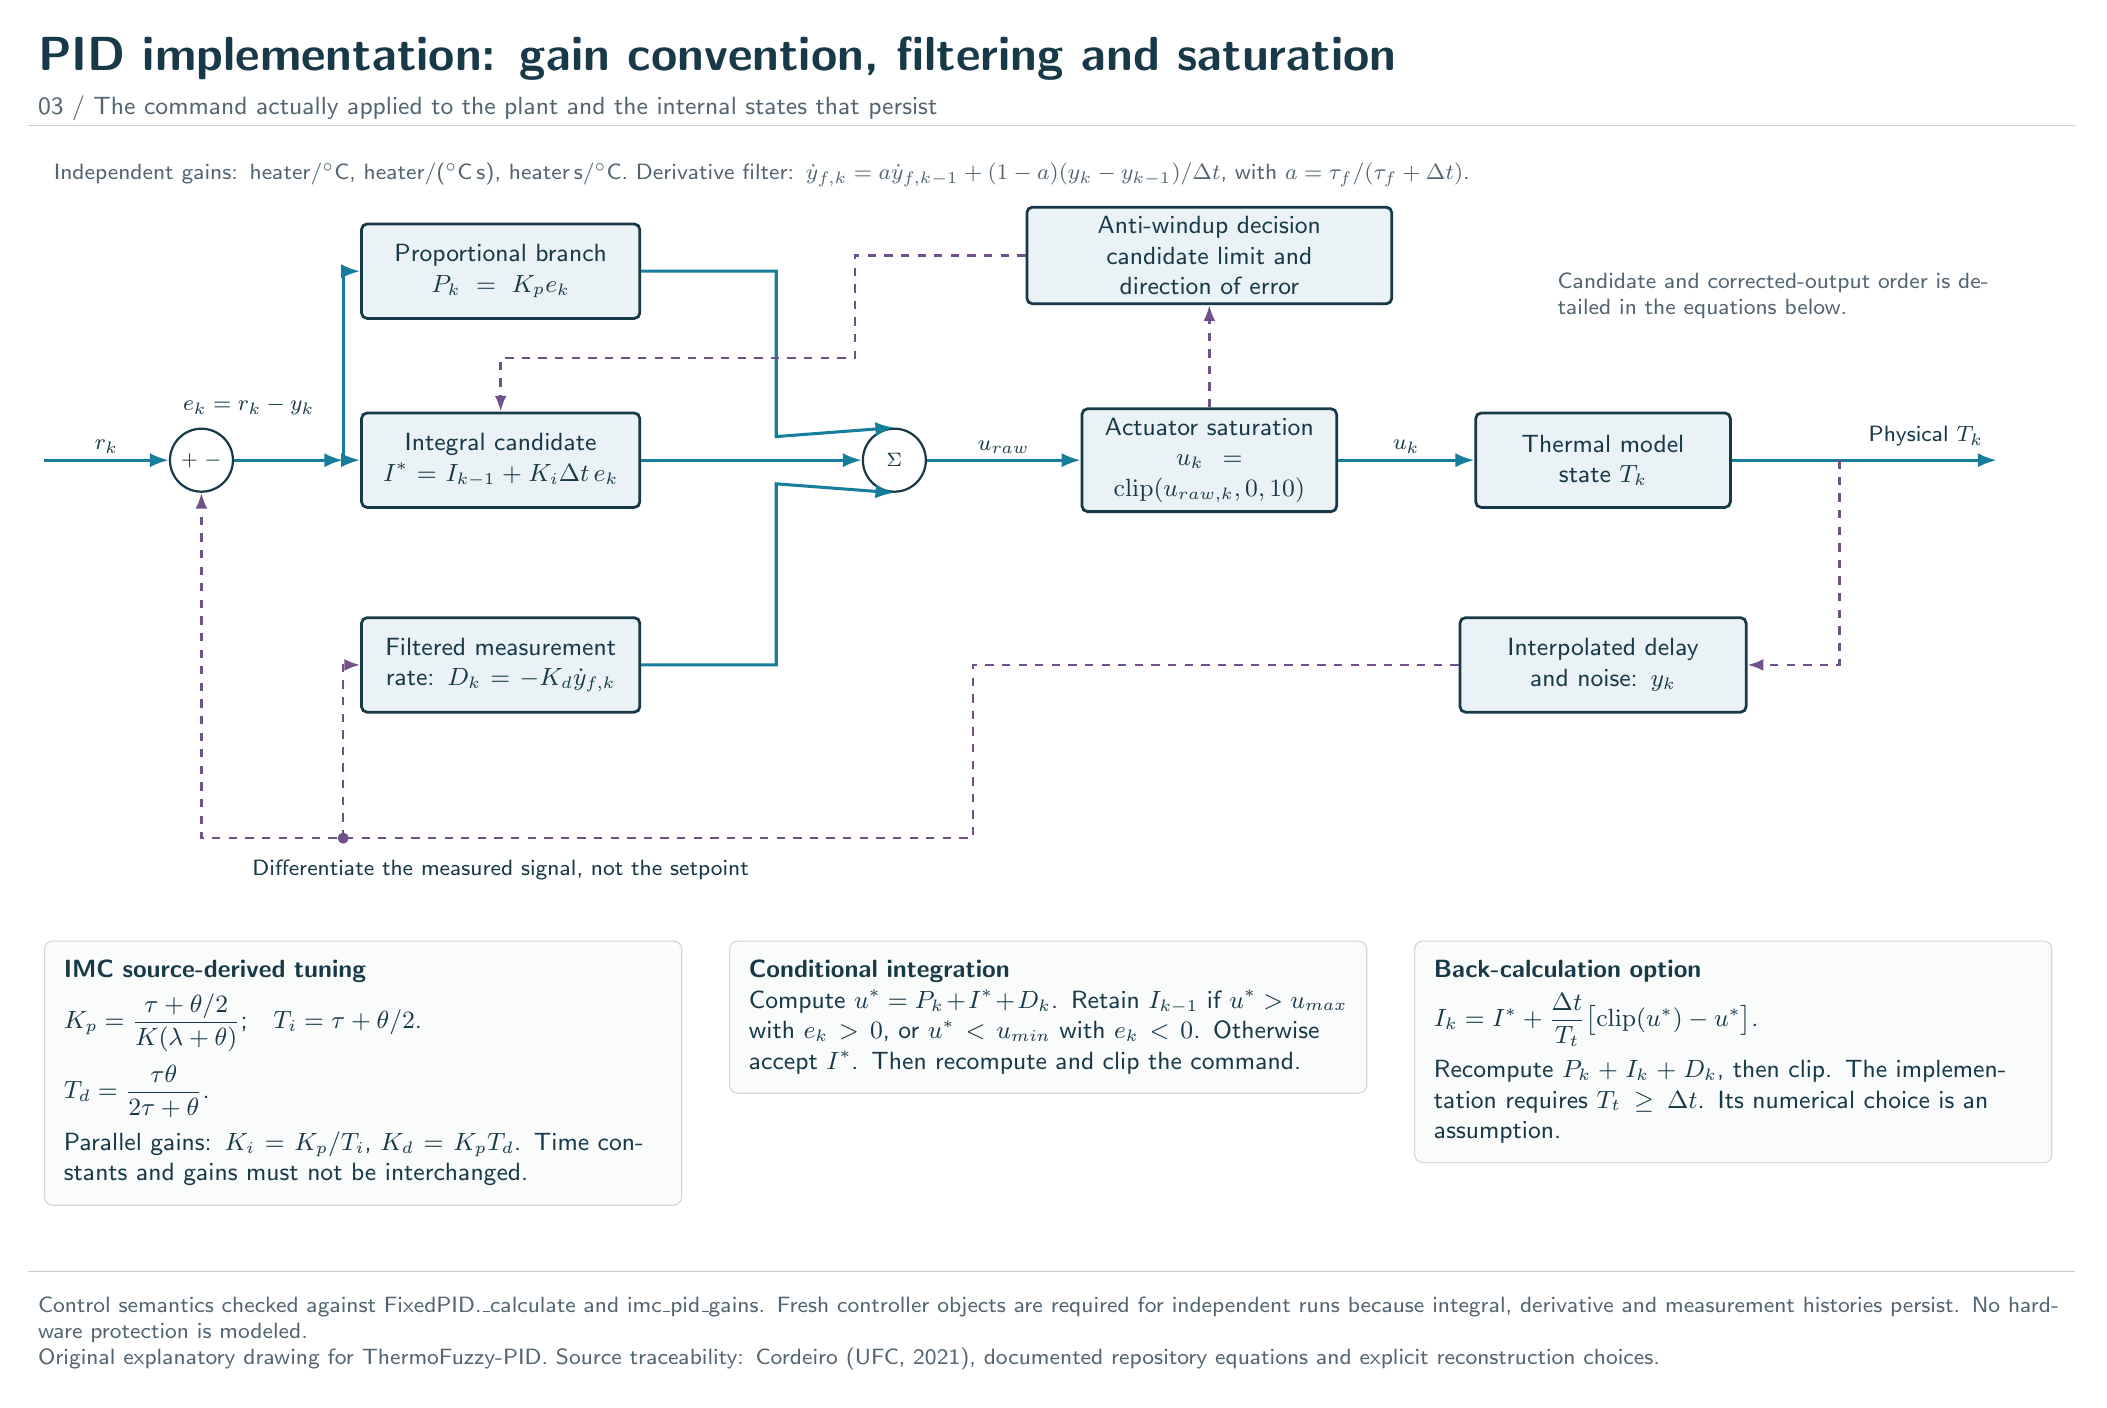
\begin{tikzpicture}[x=1cm,y=1cm]
\atlasheader{PID implementation: gain convention, filtering and saturation}{03 / The command actually applied to the plant and the internal states that persist}
\node[sensor,draw=ink] (sum)at(2.2,-5.5){$+\;-$};
\draw[process](.2,-5.5)--node[labelbox,above]{$r_k$}(sum.west);
\draw[process](sum.east)--(4,-5.5);
\node[labelbox,anchor=south]at(2.8,-5.0){$e_k=r_k-y_k$};
\node[box,text width=3.3cm] (p)at(6,-3.1){Proportional branch\\$P_k=K_p e_k$};
\node[box,text width=3.3cm] (i)at(6,-5.5){Integral candidate\\$I^*=I_{k-1}+K_i\Delta t\,e_k$};
\node[box,text width=3.3cm] (d)at(6,-8.1){Filtered measurement\\rate: $D_k=-K_d\dot y_{f,k}$};
\draw[process](4,-5.5)--(4,-3.1)--(p.west);
\draw[process](4,-5.5)--(i.west);
\node[sensor,draw=ink] (add)at(11,-5.5){$\Sigma$};
\draw[process](p.east)--(9.5,-3.1)--(9.5,-5.2)--(add.north);
\draw[process](i.east)--(add.west);
\draw[process](d.east)--(9.5,-8.1)--(9.5,-5.8)--(add.south);
\node[box,text width=3cm] (limit)at(15,-5.5){Actuator saturation\\$u_k=\mathrm{clip}(u_{raw,k},0,10)$};
\node[box,text width=3cm] (plant)at(20,-5.5){Thermal model\\state $T_k$};
\draw[process](add.east)--node[labelbox,above]{$u_{raw}$}(limit.west);
\draw[process](limit.east)--node[labelbox,above]{$u_k$}(plant.west);
\draw[process](plant.east)--(25,-5.5);
\node[labelbox,anchor=south]at(24.1,-5.4){Physical $T_k$};
\node[box,text width=3.4cm] (sense)at(20,-8.1){Interpolated delay\\and noise: $y_k$};
\draw[signal](23,-5.5)--(23,-8.1)--(sense.east);
\draw[signal](sense.west)--(12,-8.1)--(12,-10.3)--(2.2,-10.3)--(sum.south);
\draw[signal](4,-10.3)--(4,-8.1)--(d.west);
\fill[measure](4,-10.3)circle(2pt);
\node[labelbox,anchor=north]at(6,-10.5){Differentiate the measured signal, not the setpoint};
\node[box,text width=4.4cm] (aw)at(15,-2.9){Anti-windup decision\\candidate limit and direction of error};
\draw[signal](limit.north)--(aw.south);
\draw[signal](aw.west)--(10.5,-2.9)--(10.5,-4.2)--(6,-4.2)--(i.north);
\node[annotation,anchor=north west,text width=5.9cm]at(19.3,-3.0){Candidate and corrected-output order is detailed in the equations below.};
\node[panel,anchor=north west,text width=7.6cm]at(.2,-11.6){\textbf{IMC source-derived tuning}\\[3pt]
$K_p=\dfrac{\tau+\theta/2}{K(\lambda+\theta)}$;\quad $T_i=\tau+\theta/2$.\\[4pt]
$T_d=\dfrac{\tau\theta}{2\tau+\theta}$.\\[4pt]
Parallel gains: $K_i=K_p/T_i$, $K_d=K_pT_d$. Time constants and gains must not be interchanged.};
\node[panel,anchor=north west,text width=7.6cm]at(8.9,-11.6){\textbf{Conditional integration}\\Compute $u^*=P_k+I^*+D_k$. Retain $I_{k-1}$ if $u^*>u_{max}$ with $e_k>0$, or $u^*<u_{min}$ with $e_k<0$. Otherwise accept $I^*$. Then recompute and clip the command.};
\node[panel,anchor=north west,text width=7.6cm]at(17.6,-11.6){\textbf{Back-calculation option}\\[3pt]
$I_k=I^*+\dfrac{\Delta t}{T_t}\bigl[\mathrm{clip}(u^*)-u^*\bigr]$.\\[4pt]
Recompute $P_k+I_k+D_k$, then clip. The implementation requires $T_t\ge\Delta t$. Its numerical choice is an assumption.};
\node[annotation,anchor=north west,text width=25cm]at(.2,-1.6){Independent gains: heater/$^{\circ}$C, heater/($^{\circ}$C\,s), heater\,s/$^{\circ}$C. Derivative filter: $\dot y_{f,k}=a\dot y_{f,k-1}+(1-a)(y_k-y_{k-1})/\Delta t$, with $a=\tau_f/(\tau_f+\Delta t)$.};
\atlasfooter{Control semantics checked against FixedPID.\_calculate and imc\_pid\_gains. Fresh controller objects are required for independent runs because integral, derivative and measurement histories persist. No hardware protection is modeled.}
\end{tikzpicture}
\end{document}
